\section{Architecture}

\begin{figure}[H]
    \centering
    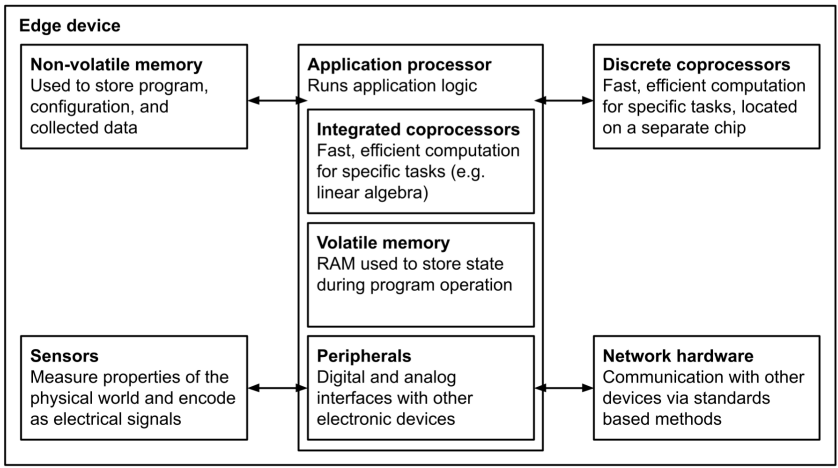
\includegraphics[width=0.5\linewidth]{images/eeai4.png}
    \caption{Hardware architecture}
\end{figure}
The hardware architecture of embedded and edge AI systems consists of several key components:
\begin{itemize}
    \item \textit{Non-volatile memeory}: used to store programs, configurations, and collected data. 
        Flash memory is typically used for this purpose, as it retains data even when the system is powered off. 
        It is ideal for storing information that does not change frequently but is slow to read and extremely slow to write.
    \item \textit{Application processor}: runs the application logic and manages program execution. 
        It includes an integrated coprocessor for efficient computation of specific tasks, volatile memory (RAM) for storing the system state during operation, and various digital and analog peripherals that allow interaction with other electronic components.
    \item \textit{Discrete coprocessors}: external chips designed for high-speed, efficient mathematical computations. 
        They provide additional processing power for specialized AI workloads that require high performance.
    \item \textit{Sensors}: measure physical-world properties and convert them into electrical signals for processing. 
        They enable real-time data collection, which is essential for AI-driven decision-making.
    \item \textit{Network hardware}:  ensures communication with other devices using standardized protocols.
        Reliable connectivity is crucial for data exchange in distributed AI systems.
\end{itemize}
\noindent RAM is often the performance bottleneck in embedded and edge AI systems. 
It is very fast but consumes significant energy, making efficiency critical in power-sensitive applications.
Since it is volatile, data is lost when power is turned off. 
RAM is also costly and takes up a large physical footprint, impacting the overall design of embedded AI devices.